
\documentclass{article}
\usepackage[utf8]{inputenc}
\usepackage[T5]{fontenc}
\usepackage{graphicx}
\usepackage[margin=1.5cm]{geometry}
\title{Lab 4: Threads}
\author{Nguyễn Thanh Hùng -- 2540056}
\date{}
\begin{document}
\maketitle
The 2D kernel maps thread $(x,y)$ to pixel $(y,x)$. The notebook compares 1D and 2D blocks with the same number of threads and plots CPU/GPU speedup.
Exercise 1: $16\times16$ permits four blocks and 1024 threads/SM; $8\times8$ permits only 512 threads with eight blocks; $32\times32$ exceeds 512 threads/block.
Exercise 2: 128, 256, 512 and 1024 threads/block give 512, 1024, 1536 and 1024 resident threads respectively. Choose 512.
Exercise 3: $\lceil2000/512\rceil512=2048$ launched threads; 48 are inactive.
These exercise limits are hypothetical; benchmarks use the actual GPU limits.

Kernel timing uses \texttt{time.time()} after JIT warm-up and CUDA synchronization,
averaged over three GPU runs. Device allocation and host/device copies are excluded.
CPU measurements are single runs. Speedup is relative to the stated CPU implementation.
Actual measurements appear after running the notebook on Colab; no timings are assumed here.
\IfFileExists{results.tex}{\begin{center}
\resizebox{\linewidth}{!}{
\begin{tabular}{lllllll}
\hline
block & cpu\_ms & gpu\_1d\_ms & gpu\_2d\_ms & speedup\_1d & speedup\_2d & max\_error \\
\hline
(8, 8) & 463.127 & 0.0768503 & 0.0572205 & 6026.35 & 8093.73 & 1 \\
(16, 16) & 463.127 & 0.0404517 & 0.0561078 & 11448.9 & 8254.22 & 1 \\
(32, 16) & 463.127 & 0.0501474 & 0.05126 & 9235.31 & 9034.86 & 1 \\
(32, 32) & 463.127 & 0.0549952 & 0.0743071 & 8421.22 & 6232.6 & 1 \\
\hline
\end{tabular}
}
\end{center}}{}
\IfFileExists{performance.png}{\begin{center}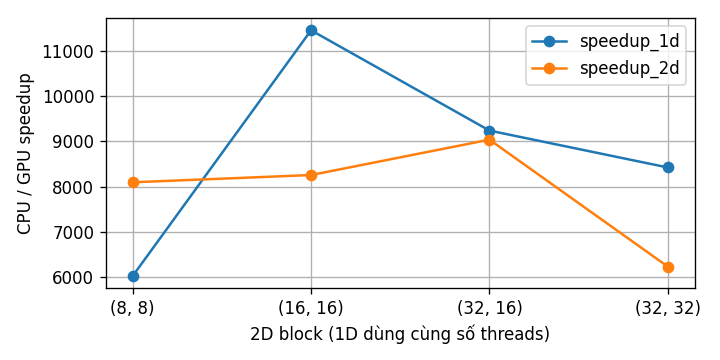
\includegraphics[width=.75\linewidth]{performance.png}\end{center}}{}
\IfFileExists{images.png}{\begin{center}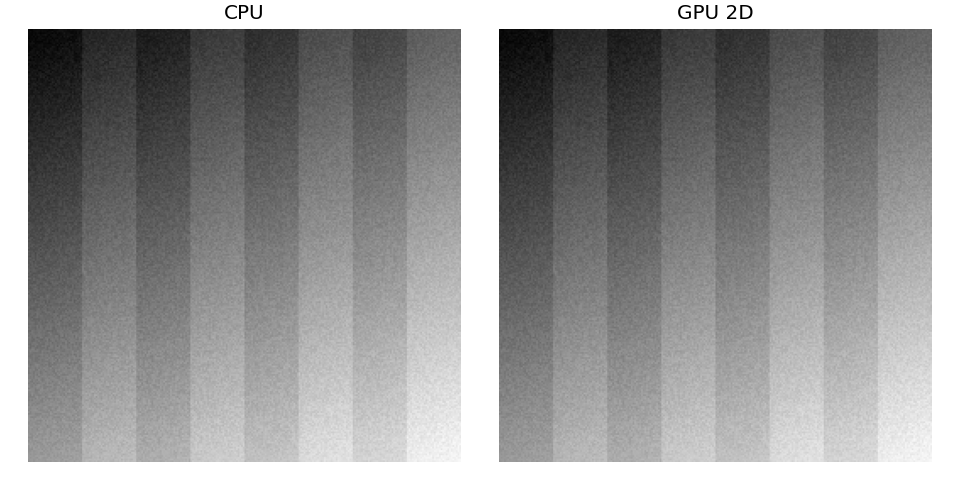
\includegraphics[width=\linewidth]{images.png}\end{center}}{}
\IfFileExists{histograms.png}{\begin{center}\includegraphics[width=.8\linewidth]{histograms.png}\end{center}}{}
\end{document}
